haiiiiiiiiii222222222222


% ======================================================================
% Chương 2
% ======================================================================
\chapter{高等教育质量保障的理论基础}
\label{chap:ly_luan}

% ======================================================================
% TRANG 1-2: GIỚI THIỆU CHƯƠNG
% ======================================================================
\section*{引言}
\addcontentsline{toc}{section}{引言}

在全球化和知识经济崛起的背景下,高等教育(GDĐH)的质量已成为决定每个国家竞争力的一个战略性因素。大学不再是与世隔绝的“象牙塔”,而已成为活跃的主体,受到来自社会、经济和政治等多重复杂压力的影响。为应对这些挑战,世界各地纷纷建立和发展了质量保障(ĐBCL)体系,特别是外部质量保障(External Quality Assurance - EQA)体系。然而,将发达国家的质量保障模式应用于像越南这样的转型经济体背景时,常会遇到诸多困难和矛盾。那些侧重于合规性控制或僵化标准的传统模式,显得不够灵活,难以解释和引导一个正处于快速发展和深刻变革阶段的高等教育体系。

这种复杂性对理论提出了一个迫切的要求:需要一个足够强大和全面的分析框架,以便能够“解剖”高等教育质量保障体系的本质。这样的理论框架不仅要能识别出影响因素,还必须能解释其动因、权力关系以及各主要主体——国家、认证机构和大学之间潜在的矛盾。现实表明,以往的许多研究通常只关注单一层面,或使用单一理论,导致了片面的看法。例如,一些研究可能很好地解释了为什么大学必须遵守国家规定,但却无法解释为什么培养方案在响应企业需求方面仍然变化缓慢。同样,一些分析侧重于问责制,却忽略了对组织行为有深远影响的文化和无形规范等因素。

这一“理论空白”正是本章的出发点。本论文认为,为了获得全面的理解,需要整合多种理论视角。具体而言,一个有效的分析框架必须能够同时解释三个核心问题:(1)为什么各大学会采用相似的质量保障结构和流程(\textit{关于合法性的问题})?(2)质量为谁定义和创造,以及如何平衡不同群体的利益(\textit{关于利益相关者的问题})?(3)采用何种机制来确保大学履行其承诺和责任(\textit{关于问责制的问题})?

为填补这一空白,本章将进行系统性的构建。\textbf{首先},本章将深入分析社会科学与公共管理的三大经典理论支柱:新制度主义、利益相关者理论和委托代理理论。分析将不仅停留在概念介绍,还将批判并指出每种理论在独立应用于高等教育领域时的局限性。\textbf{其次},本章将综述全球现代质量保障的发展趋势,特别是混合模型(Hybrid Model)和适应性框架(Adaptive Framework)的兴起,这些都是旨在超越传统理论局限的实践努力。\textbf{最后,也是最重要的},在这些分析的基础上,本章将提出并详细论证一个新的理论模型——\textbf{越南高等教育混合与适应性质量保障模型(V-AQA Model)}。该模型将作为核心的理论工具,为本论文后续章节的现状分析和方案建议提供指导和视角。


% done chuong 2 goi 1


% ======================================================================
% TRANG 3-5: THUYẾT TÂN THỂ CHẾ (PHẦN 1)
% ======================================================================
\section{质量保障体系分析的基础理论框架}
\label{sec:khung_ly_thuyet_nen_tang}

在质量保障体系中,政府、认证机构和大学之间的复杂关系可以通过多种理论视角来审视。以下三种理论提供了强大且互补的分析工具,有助于解读质量保障政策与实践背后的动因\footcite{OxfordResearch}\footcite{GovernanceTheories}\footcite{SAGE_HE}。

\subsection{新制度主义理论 (New Institutionalism Theory)}
\label{subsec:tan_the_che_nen_teng}

\subsubsection{起源与发展历史}
新制度主义(New Institutionalism)兴起于1970和1980年代,作为对纯理性经济学和组织理论的一种回应,后者认为组织行为主要由技术效率和利益最大化等因素决定。John W. Meyer、Brian Rowan,以及后来的Paul DiMaggio和Walter Powell等先驱思想家认为,组织,特别是像学校、医院这样的公共部门组织,不仅存在于经济市场中,也存在于一个更广泛的社会和文化环境中\footcite{MeyerRowan1977}\footcite{DiMaggioPowell1983}。

“旧制度主义”与“新制度主义”的核心区别在于分析的重点。旧制度主义(old institutionalism)通常关注法律、宪法和组织结构图等正式、有形的结构。相反,新制度主义(new institutionalism)将“制度”的概念扩展到包括不成文规则、社会规范、符号、认知脚本和文化模式等无形但影响强大的因素\footcite{MeyerPowell2020}。据此,一个组织之所以以某种方式行事,不仅因为法律要求(规制性因素),还因为“这是正确的做法”(规范性因素),或者仅仅因为“大家都是这么做的”(文化-认知性因素)。该理论提供了一个强大的视角来解释为什么在同一领域内的组织,例如大学,倾向于发展出极其相似的结构、流程和实践,这一现象被称为“制度同形”。

\subsubsection{核心概念及其在越南高等教育中的应用}

要将此理论应用于分析越南高等教育的质量保障体系,需要阐明三个核心概念:

\paragraph{制度场域 (Institutional Field):}
一个“制度场域”被定义为共同构成一个公认的制度生活领域的组织集合(如供应商、消费者、监管机构)\footcite{DiMaggioPowell1983}。在越南高等教育的背景下,制度场域包括一个复杂的主体网络:
\begin{itemize}
    \item \textbf{国家管理机构:} 教育培训部、其他主管部委以及地方教育培训厅。
    \item \textbf{高等教育机构:} 国家大学、区域性大学、公立大学、私立大学以及有外国因素的大学。
    \item \textbf{质量保障组织:} 国内的教育质量认证中心(如VNU-CEA)以及国际/区域性认证组织(如AUN-QA, HCERES, FIBAA)。
    \item \textbf{其他利益相关方:} 企业(雇主)、行业协会、学生、家长以及整个社会。
\end{itemize}
所有这些组织相互作用,共享一套关于“质量”的规则、规范和定义,创造了一个塑造每所大学行为的制度环境。

\paragraph{合法性 (Legitimacy):}
合法性是社会对一个组织行为的广泛认可,认为其在社会建构的规范、价值、信念和定义体系中是“可取的、正确的或适当的”\footcite{Suchman1995}。对于一所越南大学来说,获得并维持合法性至关重要,因为它能带来具体的利益:
\begin{itemize}
    \item \textbf{获取资源:} 获得质量认可的学校更容易获得国家预算、吸引企业项目和其他资助。
    \item \textbf{吸引优秀学生:} 来自认证机构的声誉和认可是吸引学生和家长的关键因素。
    \item \textbf{稳定与生存:} 在竞争环境中,被视为“合法”有助于学校巩固地位并确保可持续生存。
\end{itemize}
因此,参与认证等质量保障活动不仅是一项技术活动,也是寻求和巩固合法性的重要战略。

\paragraph{制度同形 (Institutional Isomorphism):}
这是指同一制度场域内的组织变得越来越相似的过程。DiMaggio和Powell(1983)指出了导致同形的三个主要机制,这三个机制在越南高等教育的质量保障体系中都可以清晰地观察到\footcite{DiMaggioPowell1983}。

\textbf{1. 强制性同形 (Coercive Isomorphism):} 这是来自一个组织所依赖的其他组织的正式和非正式压力的结果。在越南的背景下,这是最强大的机制,体现在:
\begin{itemize}
    \item \textit{法律规定:} 《高等教育法》、教育培训部的法令和通知要求各大学必须每五年参加一次质量认证。不遵守规定可能导致不被批准开设新专业或减少招生名额等制裁。
    \item \textit{主管机构的压力:} 主管部委或省人民委员会也对质量和排名提出要求,迫使下属学校遵守一个共同的框架。
    \item \textit{资源依赖:} 质量保障的要求通常与国家预算的分配或参与国家重点项目(如关于培养博士师资的89号提案)挂钩。
\end{itemize}
其结果是,越南大多数大学都必须建立质量保障单位,按照国家规定的统一脚本执行自评过程并参与外部认证。


% done chuong 2 goi 1 v2


Chắc chắn rồi, đây là nội dung đã được dịch sang tiếng Trung và định dạng lại theo yêu cầu của bạn:

% ======================================================================
% TRANG 6-7: THUYẾT TÂN THỂ CHẾ (PHẦN 2)
% ======================================================================

\paragraph{2. 模仿性同形 (Mimetic Isomorphism):}
该机制产生于组织面临不确定性(uncertainty)之时。当目标不明确或环境过于复杂时,组织倾向于模仿同一领域内被它们认为更成功或更具合法性的其他组织\footcite{DiMaggioPowell1983}。这是一种降低风险并快速获得认可的策略。在越南高等教育的背景下,这种现象非常普遍:
\begin{itemize}
    \item \textit{培养方案的模仿:} 许多新成立的大学或地方院校在构建其培养方案时,通常会参考甚至复制顶尖大学(如河内国家大学、胡志明市国家大学或河内理工大学)的课程结构。这种行为不仅有助于节省开发课程的时间和资源,更重要的是,它创造了一种“安全”和“正确”的感觉,因为它们正走在成功者的道路上。
    \item \textit{治理模式的模仿:} 质量管理模式的应用、质量保障部门的结构设置或内部报告系统等,通常是各学校相互学习的对象。一个在某所大学成功实施的模式会迅速成为其他学校效仿的“典范”,从而在管理实践中掀起一股同步化的浪潮。
\end{itemize}
关于“何为国际一流大学”或“何为有效的质量保障体系”的不确定性,正是模仿性同形得以蓬勃发展的沃土。

\paragraph{3. 规范性同形 (Normative Isomorphism):}
该机制主要源于专业化(professionalization)过程\footcite{DiMaggioPowell1983}。当一个行业发展时,它会通过以下渠道形成一套共同的规范、价值观和工作方法:
\begin{itemize}
    \item \textit{专业培训:} 这是在质量保障领域影响最强的渠道。越南各大学的认证专家、质量保障负责人通常会参加由国家认证中心或东盟大学网络(AUN)等区域组织举办的培训课程。在这些课程中,他们学习同一套标准(例如,AUN-QA标准),实践同一套评估方法。回到学校后,他们带来并应用这些共同的规范,逐渐使不同学校的质量保障实践变得相似\footcite{AUN-QAGuide}。
    \item \textit{专业网络:} 专家网络、协会(如越南大学与学院协会)以及关于质量保障的科学研讨会的发展,创造了一个让职业规范得以传播和巩固的空间。“最佳实践”(best practices)被分享并迅速成为全行业的非官方标准。
    \item \textit{人员招聘与流动:} 招聘在先进教育体系中受过培训的教师,或管理人员在各校之间的调动,也是传播管理和质量保障规范的一个渠道。
\end{itemize}

\subsubsection{新制度主义理论的应用与批判}

通过新制度主义的视角来分析越南高等教育的质量保障体系可以发现,该体系的形成和运作是一个复杂的过程,由三种同形机制的相互作用所塑造。各大学不仅单纯遵守教育培训部的规定(强制性),还主动学习其他学校的模式(模仿性),并受到质量保障专家社群共同规范的影响(规范性)。

然而,对新制度主义最大的批判之一是其倾向于过分强调合规性和环境压力,有时会轻视组织自身的主动性和创新能力(institutional agency)。该理论很好地解释了为什么组织会变得相似,但却较少解释为什么某些组织能够采取突破性、创造性的举措,或者有能力进行“脱钩”(decoupling)——即形式上采纳所要求的结构和流程以获得合法性,而内部核心活动却保持不变\footcite{MeyerRowan1977}。

此外,新制度主义未能提供一个足够强大的工具来分析大学如何处理和平衡来自同一制度场域内不同群体的矛盾压力。例如,来自政府的压力可能是提升服务地方产业的能力,而来自国际学术界的压力则是增加在ISI/Scopus期刊上的发表。要理解这种拉锯和利益协商过程,我们需要借助另一种理论视角:利益相关者理论。

\subsection{利益相关者理论 (Stakeholder Theory)}
\label{subsec:ben_lien_quan_nen_tang}

\subsubsection{起源与核心原则}

由R. Edward Freeman在其经典著作《战略管理:一种利益相关者的方法》(1984)中系统发展的利益相关者理论,在管理思维上掀起了一场革命。该理论作为对传统管理模式(仅关注股东利益)的回应而诞生。Freeman认为,一个组织的可持续成功,不能仅通过最大化股东利润来实现,而必须为所有能够影响或被组织目标实现所影响的个人和群体创造并分配价值。这些个人和群体被称为“利益相关者”(stakeholders)\footcite{Freeman1984}。

该理论已被广泛扩展并应用于不存在“股东”概念的公共和非营利组织中。在高等教育领域,它尤为适用,因为大学有众多利益诉求多样且时而冲突的利益相关者\footcite{Langrafe2020}。后续的研究系统化了基于该理论的治理核心原则,包括\footcite{LangrafeEUR2020}\footcite{IJLTER2024}:
\begin{enumerate}
    \item \textbf{参与 (Participation):} 利益相关者需要积极参与到影响他们的决策过程中。
    \item \textbf{信息交换 (Information Exchange):} 需要有机制让组织倾听利益相关者的要求,同时透明地通报其活动和决策。
    \item \textbf{信任 (Trust):} 建立基于相互信任和尊重的关系是有效合作的基础。
    \item \textbf{战略规划 (Strategic Planning):} 利益相关者的利益和要求必须被整合到组织的战略规划过程中。
\end{enumerate}

\subsubsection{越南高等教育质量保障中的利益相关者地图}

要将此理论应用于具体情境,首要且最重要的一步是识别(mapping)越南高等教育质量保障体系中的利益相关者并分析他们的利益(stake)。这样的地图有助于明确质量保障体系需要服务的对象群体。
\begin{figure}[h!]
    \centering
    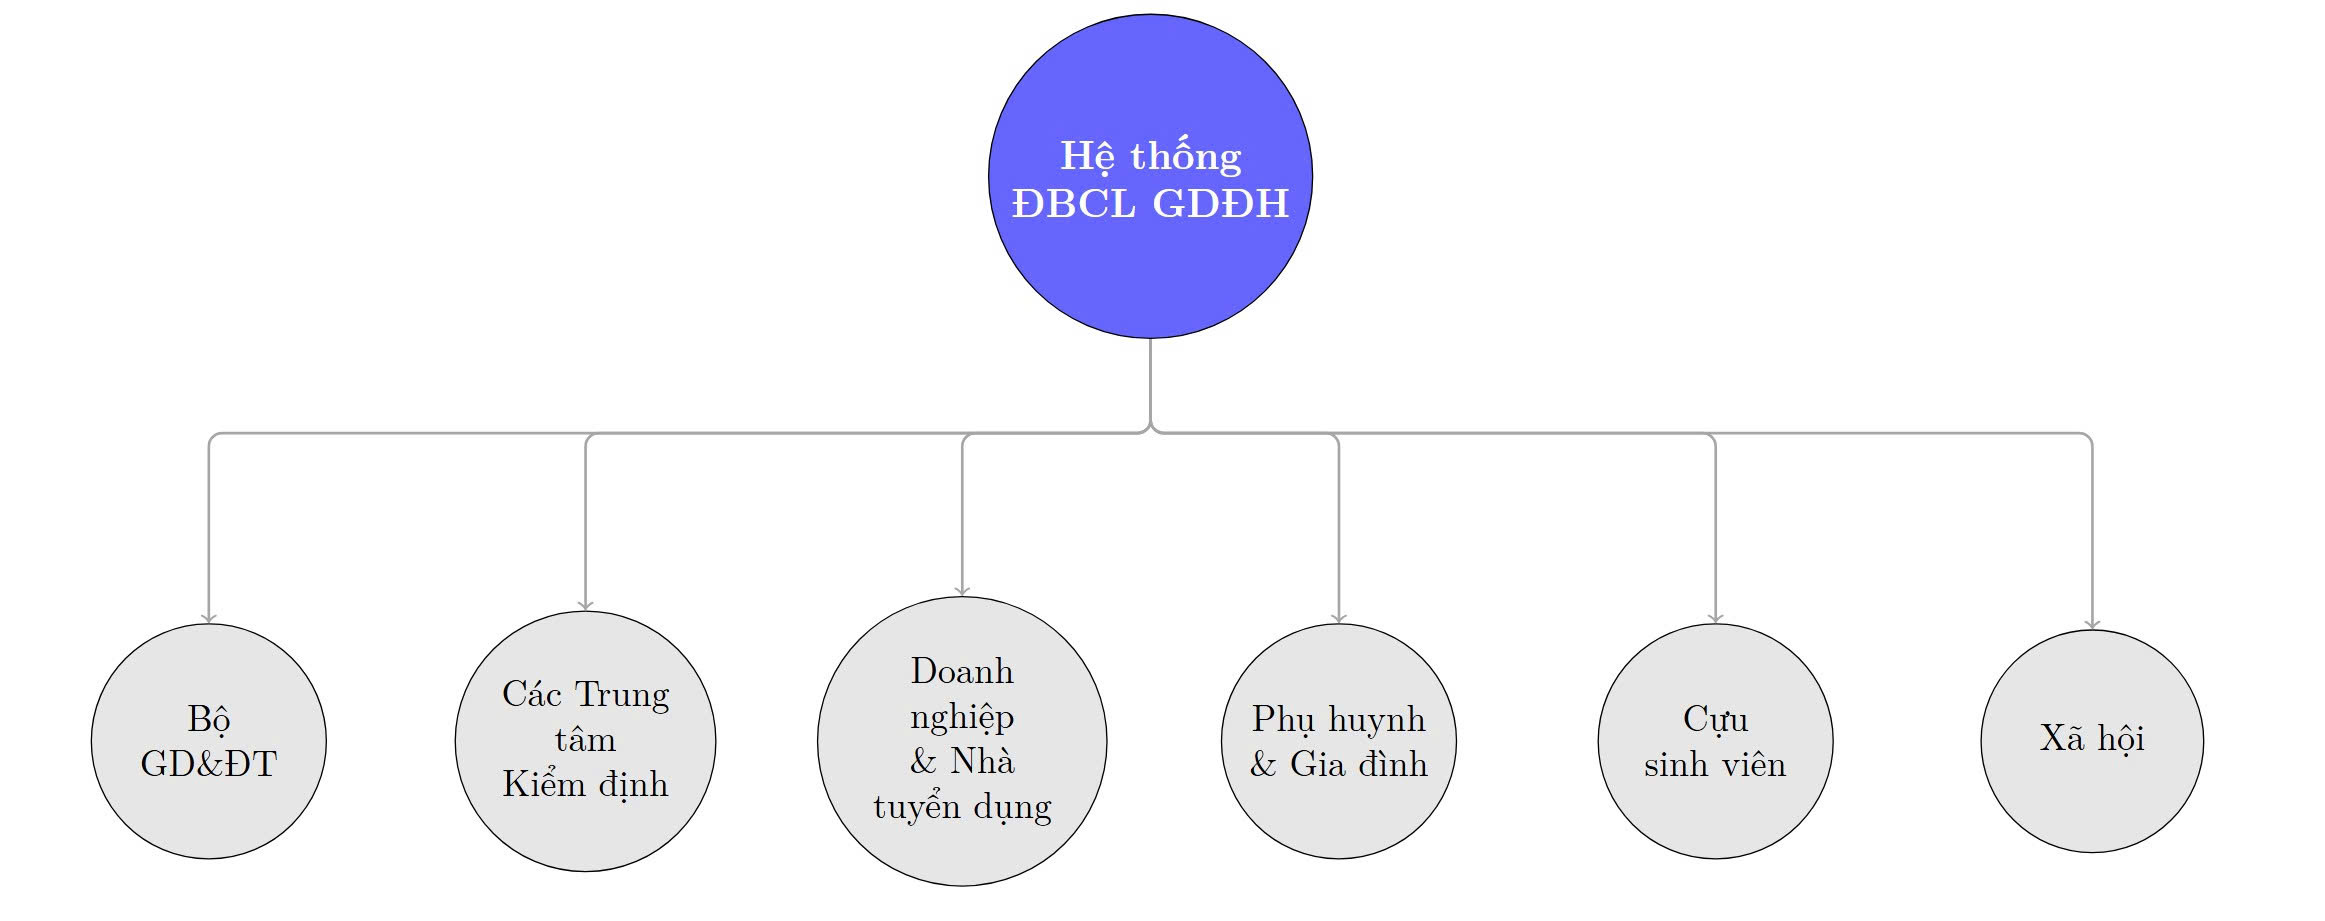
\includegraphics[width=\textwidth]{image/stakeholder_map.jpg} 
    \caption{越南高等教育质量保障体系中的利益相关者地图}
    \label{fig:stakeholder-map}
\end{figure}

\begin{itemize}
    \item \textbf{内部利益相关者 (Internal Stakeholders):}
        \begin{itemize}
            \item \textit{学校领导层(校董会、校领导班子):} 主要利益是学校的声誉、财务稳定、达成KPI指标以及遵守上级规定。
            \item \textit{教师与研究人员:} 利益包括学术自由、良好的工作条件、专业发展机会以及减少行政负担。
            \item \textit{行政人员(包括质量保障处干部):} 利益是流程清晰、有足够资源完成工作以及得到其他部门的合作。
            \item \textit{学生:} 核心利益是培养方案的质量、有效的教学方法、良好的学习环境、毕业后的就业机会以及合理的学费。
        \end{itemize}
    \item \textbf{外部利益相关者 (External Stakeholders):}
        \begin{itemize}
            \item \textit{教育培训部:} 利益是确保高等教育体系稳定运行、质量均衡,满足国家经济社会发展目标,并向政府和社会履行问责。
            \item \textit{教育质量认证中心:} 利益是维持其组织的声誉、专业性和独立性;完成被赋予的认证任务。
            \item \textit{企业与雇主:} 利益是能够招聘到具备与工作要求直接匹配的技能和知识的人力资源,减少再培训成本。
            \item \textit{家长与家庭:} 利益是为子女的投资(时间、金钱)带来应有的回报(孩子有好工作、成才)。
            \item \textit{校友:} 利益是学位证书的价值和母校声誉的提升,从而在职业网络中产生自豪感和机会。
            \item \textit{社会:} 利益是高等教育有助于创造一个公平、进步的社会,提供高质量的人力资源并维护文化价值观。
        \end{itemize}
\end{itemize}
该地图显示,质量保障体系必须服务于一个极其多样化的利益网络。一个质量改进的决策,例如增加学生的实践要求,可能会受到企业的欢迎,但却可能遭到教师(因工作量增加)或财务部门(因成本增加)的反对。识别和分析这些潜在的利益冲突,是构建一个有效的质量保障体系的第一步。



% done chuong 2 goi 2

Chắc chắn rồi, đây là nội dung đã được dịch sang tiếng Trung và định dạng lại theo yêu cầu của bạn:

% ======================================================================
% TRANG 11-13: THUYẾT CÁC BÊN LIÊN QUAN (PHẦN 2)
% ======================================================================

\subsubsection{利益相关者的显著性 (Stakeholder Salience)}

识别利益相关者仅仅是第一步。治理中的一个巨大挑战是如何处理来自这些群体的多样且常常相互矛盾的要求。并非所有利益相关者都具有同等的影响力。Mitchell, Agle和Wood(1997)提出了一个极具影响力的模型,用以确定利益相关者的“显著性”(salience),该模型基于三个核心属性\footcite{Mitchell1997}:

\begin{enumerate}
    \item \textbf{权力 (Power):} 利益相关者将其意志强加于组织之上的能力,迫使组织去做那些若无此压力则不会做的事情。权力可以来自对关键资源(如预算)的控制、颁布法规的能力或影响媒体的能力。
    \item \textbf{合法性 (Legitimacy):} 社会承认某一利益相关者的要求或行动在特定社会背景下是正当、适宜和正确的。合法性来自法律规定、合同或社会道德规范。
    \item \textbf{紧迫性 (Urgency):} 利益相关者的要求需要立即关注的程度。紧迫性取决于两个因素:时间敏感性(若不及时处理,要求将失去价值)和该要求对利益相关者的重要程度。
\end{enumerate}

根据拥有一、二或全部三个属性,利益相关者可被划分为不同优先级的群体,从“潜在”群体(latent stakeholders,仅有1个属性)到需要领导层最多关注的“决定性”群体(definitive stakeholders,拥有全部3个属性)。

将此模型应用于越南高等教育的质量保障体系,我们可以解释一些重要现象:
\begin{itemize}
    \item \textbf{教育培训部}是一个“决定性”利益相关者。该部拥有\textit{权力}(通过分配预算、颁发许可),拥有\textit{合法性}(依据《高等教育法》),并且其要求通常具有\textit{紧迫性}(与认证、报告周期挂钩)。因此,该部的声音分量最重,各大学通常优先满足其要求。
    \item \textbf{企业/雇主}是一个拥有\textit{合法性}(他们有权要求高质量的人力资源)和\textit{紧迫性}(人力需求不断变化)的利益相关者,但却缺乏直接\textit{权力}来迫使大学立即改变培养方案。这解释了为什么尽管企业不断抱怨学生质量,但大学培养方案的变革仍然缓慢。
    \item \textbf{学生和家长}拥有很高的\textit{合法性}和\textit{紧迫性},但他们的权力是分散的。只有当他们的要求通过大规模调查或媒体汇集起来时,他们的权力才会变得更加显著。
\end{itemize}
因此,显著性模型帮助我们理解,质量保障过程并非一个所有声音都平等的绝对民主过程,而是一个“政治舞台”,各大学必须不断权衡并优先考虑来自最具影响力的利益相关者的要求。

\subsubsection{利益相关者理论的应用与批判}

利益相关者理论提供了一个有效的分析工具,用以解读质量保障体系中的利益冲突。它有助于回答“质量为谁服务?”这一问题。通过识别利益相关者并分析其优先级,我们可以理解为什么质量的某些方面(例如:国际论文发表数量)会比其他方面(例如:学生的实践技能)更受重视。

然而,该理论也有其局限性。应用它时最大的挑战在于,当利益相互冲突时,如何找到一个最优方案来\textbf{平衡}这些利益。例如,为满足企业要求而加强实践教学会增加培养成本,可能导致学费上涨,从而引起学生和家长的反对。利益相关者理论很好地描述了这场争论,但并未提供解决它的明确公式。此外,该理论侧重于有形的关系和利益,但较少关注对组织行为有强大影响的无形文化规则和规范——而这正是新制度主义理论的长处。要理解具体的问责机制,我们需要借助第三种理论。

\subsection{委托代理理论 (Principal-Agent Theory)}
\label{subsec:uy_nhiem_nen_tang}

\subsubsection{起源与核心概念}
委托代理理论起源于经济学,特别是金融经济学和公司理论,其基础性工作由Stephen Ross等学者,特别是Michael Jensen和William Meckling在1970年代完成\footcite{JensenMeckling1976}。该理论旨在分析在一方(委托人 - Principal)雇佣或委托另一方(代理人 - Agent)代其执行某项工作时所产生的问题。

这种关系的核心问题(代理问题)源于两个基本条件:
\begin{enumerate}
    \item \textbf{目标冲突 (Conflict of Interest):} 委托人和代理人的利益并非总是一致。例如,股东(委托人)希望最大化利润,而管理者(代理人)可能希望最大化权力或其他个人利益。
    \item \textbf{信息不对称 (Information Asymmetry):} 代理人通常比委托人拥有更多关于工作及自身努力的信息。委托人难以完美地监督代理人的每一个行动。
\end{enumerate}
这两个条件的结合产生了两种主要风险\footcite{Eisenhardt1989}:
\begin{itemize}
    \item \textbf{道德风险 (Moral Hazard):} 合同签订后,由于委托人无法观察其努力程度,代理人可能不会尽全力工作。例如,一所大学(代理人)在从政府(委托人)获得预算后,可能不会尽最大努力投入于改进教学质量。
    \item \textbf{逆向选择 (Adverse Selection):} 签订合同前,代理人可能隐瞒信息或歪曲自身能力以求被选中。例如,一所大学可能会“美化”其自评报告,以获得认证机构的承认。
\end{itemize}
为解决这些问题,该理论提出了设计有效合同、创建激励机制(incentives)以协调利益等解决方案,最重要的是,建立\textbf{监督与报告系统(monitoring and reporting systems)}以减少信息不对称。


% done chuong 2 goi 3

Chắc chắn rồi, đây là nội dung đã được dịch sang tiếng Trung và định dạng lại theo yêu cầu của bạn:

% ======================================================================
% TRANG 16-18: THUYẾT ỦY NHIỆM (PHẦN 2) VÀ PHÊ PHÁN
% ======================================================================

\subsubsection{作为监督和合同机制的质量保障体系}

从委托代理理论的视角来看,整个外部质量保障体系可以被视为一个复杂的监督和合同机制,旨在解决“代理问题”。

\paragraph{多层次的委托代理关系:}
在高等教育中,关系不仅仅是单个委托人与代理人之间的关系。它是一系列相互嵌套的委托代理关系链,使得管理和监督变得复杂\footcite{Borgos2013}。我们可以将越南的这一关系链想象如下:
\begin{itemize}
    \item \textbf{第一层(政府 $\rightarrow$ 教育培训部):} 政府(委托人)将管理和发展国家高等教育体系的任务交给教育培训部(代理人)。
    \item \textbf{第二层(教育培训部 $\rightarrow$ 大学):} 教育培训部(委托人)向各大学(代理人)颁发办学许可并分配预算,期望各大学能够培养出高质量的人力资源并执行服务社会的研究任务。
    \item \textbf{第三层(校领导班子 $\rightarrow$ 院/系):} 校领导班子(委托人)将招生指标和预算分配给各院系(代理人),要求各院系保证其单位的培养和研究质量。
    \item \textbf{第四层(院/系 $\rightarrow$ 教师):} 院长/系主任(委托人)将教学任务分配给每位教师(代理人),并期望他们能以最佳方式完成授课。
\end{itemize}
这一委托代理链的存在解释了为什么来自最高层(政府)的要求在传达到下层时常常会被“干扰”或变形。

\paragraph{质量保障实践中的监督机制:}
为了在上述关系链中最大限度地减少道德风险和逆向选择,质量保障体系发展出了多种具体的监督机制:
\begin{itemize}
    \item \textbf{报告系统 (Reporting Systems):} 自评报告、年度报告、数据统计等要求,正是上级委托人收集下级代理人活动信息的工具。
    \item \textbf{外部认证 (External Accreditation):} 这是一种专门且正式的监督形式。认证机构(如VNU-CEA或AUN-QA)扮演着第三方“审计员”的角色,受委托人(教育培训部)信任,以核实信息并评估各大学(代理人)的活动\footcite{Borgos2013}。这一过程显著减少了信息不对称。
    \item \textbf{基于成果的合同 (Outcome-based Contracts):} 尽管在越南尚不普遍,但世界范围内的趋势是将预算分配与具体的产出结果(例如:学生就业率、国际发表数量)挂钩。这是一种旨在协调委托人与代理人利益的合同形式。
    \item \textbf{声誉建设 (Reputation Building):} 排名系统和公开认证结果也是一种监督机制。一所学校(代理人)的声誉成为一项重要资产,为了保护这项资产,他们有动力按照各委托人(学生、社会)的期望行事。
\end{itemize}

\subsubsection{委托代理理论的应用与批判}

委托代理理论提供了一套锐利的分析工具,用以剖析质量保障体系中的问责结构和监督机制。它逻辑地解释了为何需要报告、检查、定期认证等流程。特别是在分析合同性关系,如国家与被赋予自主权的公立大学之间的关系时,它尤其有用。

然而,机械地将委托代理理论应用于高等教育领域也有其显著的局限性\footcite{RIHE2022}:
\begin{itemize}
    \item \textbf{过分简化目标:} 该理论假设委托人的目标可以被明确定义。但在高等教育中,“质量”是一个多维度且难以衡量的概念。政府的目标可能是发展经济,而社会的目标是公平,学术界的目标则是创作自由。谁才是真正的“委托人”?
    \item \textbf{忽略文化与规范因素:} 该理论认为主体之间的关系主要基于经济利益和理性计算。它无法解释信任、共同价值观以及职业规范(例如:教师道德)在调节教师和学校行为中的作用。
    \item \textbf{难以应用完美的合同:} 在现实中,很难设计一个能预见所有情况并准确衡量代理人所有努力的合同。教育的“产品”(人)是极其复杂的,不能像工业产品那样容易衡量。
\end{itemize}
正因为这些局限性,分析质量保障体系不能仅仅依赖委托代理理论。必须将其与新制度主义理论(以理解无形规则)和利益相关者理论(以理解多样化利益)相结合,才能获得更全面、更准确的图景。

% ======================================================================
% TRANG 19-20: CÁC MÔ HÌNH ĐBCL HIỆN ĐẠI
% ======================================================================
\section{世界现代质量保障模型}
\label{sec:mo_hinh_hien_dai_the_gioi}

治理理论的发展和实践中的挑战,推动了日益精密的质量保障模型的诞生。这些模型不再固守单一理论,而是对传统方法的局限性进行综合和超越的努力。其中,混合模型和适应性框架这两个突出的趋势,对越南具有重要的参考意义\footcite{HybridModel2023}\footcite{AdaptiveQA2022}。

\subsection{混合模型 (Hybrid Model): 协调问责与改进}

\subsubsection{诞生背景与理念}
传统的质量保障体系通常陷入两个极端之一。一是,体系过分注重对外部的\textbf{问责制(accountability)}(自上而下),导致学校只专注于形式上、应付性地遵守规定,形成一种“合规文化”(culture of compliance)而非实质性改进。这是一种接近委托代理理论思维的模式。二是,体系过分注重\textbf{内部改进(improvement)}(自下而上),将全部权力交给单位自行评估,导致缺乏共同标准且难以确保对社会的问责。

混合模型应运而生,旨在解决这种紧张关系\footcite{EUA_Integration}。其理念是承认并整合这两个目标。它认为一个可持续的质量保障体系必须既能满足外部的控制和透明度要求,又能激发内部的改进动力和发展质量文化。混合模型不将问责与改进视为对立的目标,而是视其为一枚硬币的两面,相辅相成。例如,外部透明的问责要求可以为推动内部改进努力提供必要的数据和压力。反之,强大的内部改进文化将使学校更容易满足并超越外部的问责要求。

\subsubsection{组成部分与特点}
一个典型的混合模型通常具有以下特点:
\begin{itemize}
    \item \textbf{双重标准框架:} 体系可能包括一套用于问责目的的强制性\textbf{最低标准(minimum standards)},以及一套用于改进目的的鼓励性\textbf{提升标准(enhancement standards)}。
    \item \textbf{嵌套流程:} 外部认证活动的设计不仅旨在检查合规性,还旨在提供建设性建议,支持学校的改进过程。反之,内部自评和改进活动的结果被用作外部认证轮次中的重要证据。
    \item \textbf{质量保障机构的灵活角色:} 外部质量保障机构不仅扮演“裁判员”的角色,还扮演“伙伴”、“顾问”的角色,在改进过程中为学校提供支持。
\end{itemize}
欧洲质量保障体系的经验,尤其是在博洛尼亚进程之后,显示出向混合模型转变的明显趋势,其中认证流程越来越被设计为服务于质量提升的目标(enhancement-led accreditation)\footcite{EUA_Integration}。越南的实践,既要满足教育培训部的国家标准,又要参与如AUN-QA等区域认证项目,也正显示出一种混合模型正在逐渐形成的迹象,尽管可能尚非完全自觉\footcite{VNU-CEA2023}\footcite{HangNguyen2017}。

% done chuong 2 goi 4



% ======================================================================
% TRANG 21-22: KHUNG THÍCH ỨNG
% ======================================================================

\subsection{适应性框架 (Adaptive Framework): 在变化世界中的质量管理}
\label{subsec:khung_thich_ung}

\subsubsection{与传统方法的比较}
如果说混合模型解决了质量保障\textit{目标}的矛盾,那么适应性框架则解决了在不稳定和复杂环境中\textit{实施流程}的问题。传统的项目管理方法,通常被称为“瀑布模型”(Waterfall Model),遵循一个严格的线性序列:规划 → 设计 → 执行 → 测试 → 交付。该模型假设所有要求和条件都可以从一开始就明确确定,并且在整个过程中环境不会改变。

然而,在高等教育的现实中,尤其是在越南,情况则完全不同。教育部的政策可能改变,劳动力市场的需求波动,教育技术发展迅速,学校的资源也不稳定。采用一个僵化的、长达5年的瀑布式质量保障计划,通常会导致计划在尚未执行完毕时就已经过时。

适应性框架(Adaptive Framework),其源于敏捷软件开发(Agile)领域,正是为了解决这些问题而生\footcite{Wysocki2009}。它不是试图从一开始就制定一个完美的计划,而是将项目分解为短期的、重复的周期。在每个周期结束时,项目团队将重新评估结果,收集反馈,并为下一个周期调整计划。

\subsubsection{适应性框架的核心原则}
一个具有适应性的质量保障框架将基于以下原则运作:
\begin{itemize}
    \item \textbf{迭代学习 (Iterative Learning):} 整个质量保障流程被视为一个学习过程。学校可以不必每5年进行一次大型评估,而是可以针对具体方面(如教学方法、学生服务)进行更小规模的评估周期(例如,每年一次)。每个周期的结果将为改进下一个周期提供信息。
    \item \textbf{反馈循环 (Feedback Loops):} 该框架创建了快速且频繁的反馈循环。学校不必等到5年周期结束才有认证报告,而是可以在每学期或每学年后与学生、教师和企业组织反馈会议。
    \item \textbf{增量发展 (Incremental Development):} 质量改进不必同时进行,而是可以分阶段、逐步实施。例如,第一年,学校可以集中改进学生意见收集系统;第二年,专注于创新学习成果评估方法。
    \item \textbf{价值驱动的优先级排序 (Value-driven Prioritization):} 在每个周期,改进活动将根据其在当时为最重要利益相关者带来的价值来进行优先排序。
\end{itemize}

\subsubsection{对越南国情的适用性}
认为适应性框架特别适合越南国情的论点基于以下原因:
\begin{itemize}
    \item \textbf{动态的政策环境:} 越南关于高等教育的法规和政策可能会迅速变化。一个适应性框架允许学校灵活调整其质量保障策略,以适应新的要求,而无需推翻整个旧计划。
    \item \textbf{资源限制:} 学校不必投入巨额资金进行全面改革,而是可以根据其在每个阶段的有限资源,进行小规模、渐进式的改进。
    \item \textbf{逐步建立能力:} 立即实施一个复杂的质量保障体系可能会给人力团队带来过重负担。适应性框架允许学校边做边学,逐步且可持续地建立质量保障能力。
\end{itemize}
因此,将混合模型的理念与适应性框架的流程相结合,将创造出一种在目标上全面、在实施方式上灵活且务实的质量保障方法。这正是为越南构建建议模型的基础。

% ======================================================================
% TRANG 23-25: ĐỀ XUẤT MÔ HÌNH V-AQA
% ======================================================================
\section{为越南高等教育提出分析模型:混合与适应性模型 (V-AQA)}
\label{sec:mo_hinh_V-AQA_de_xuat}

\subsection{建立一个综合模型的必要性论证}
\label{subsec:luan_giai_V-AQA}
通过以上各部分的分析可以看出,使用单一理论来分析越南高等教育的质量保障体系是不全面的,并可能导致片面的结论。
\begin{itemize}
    \item \textbf{如果仅使用新制度主义},我们将能解释为何各学校会形式化地遵守规定,但难以解释来自内部的实质性改进努力或利益冲突。
    \item \textbf{如果仅使用利益相关者理论},我们将能看到利益多样化的图景,但却缺乏分析工具来解释为何某些方面的声音比其他方面更有分量,也无法解释报告和监督机制。
    \item \textbf{如果仅使用委托代理理论},我们将能清晰理解问责结构,但却会忽略文化、规范因素以及无法简化为单纯合同的复杂合作关系。
\end{itemize}

因此,越南的国情需要一个综合的分析框架,一个能够融合不同视角的模型。本论文提出了这样一个模型,名为\textbf{越南高等教育混合与适应性质量保障模型(The Vietnam - Adaptive Quality Assurance Model,简称 V-AQA)}。

该模型具有\textbf{混合性(Hybrid)},因为它承认并试图协调两个并行且时而矛盾的目标:
\begin{enumerate}
    \item \textbf{对外部的问责制(External Accountability):} 满足教育培训部、认证机构和社会的要求,以获得合法性和资源(反映了新制度主义和委托代理理论的视角)。
    \item \textbf{来自内部的改进(Internal Improvement):} 为内部利益相关者(学生、教师)创造价值,并推动一种内生的质量文化(反映了利益相关者理论的视角)。
\end{enumerate}

同时,该模型具有\textbf{适应性(Adaptive)},因为它在实施过程中强调灵活性,允许大学根据反馈和环境变化,以短期周期调整其质量保障活动,而不是遵循一个僵化的五年计划。

\subsection{V-AQA模型的结构与核心要素}
\label{subsec:cau_truc_V-AQA}

V-AQA模型的结构如同一座神殿,以理论为基石,以最终目标为屋顶,并由五个核心要素作为五根支柱支撑。这五个要素并非独立运作,而是相互作用、相互巩固,形成一个稳固的系统(见图 \ref{fig:v-aqa-model-detailed})。

\begin{figure}[h!]
    \centering
    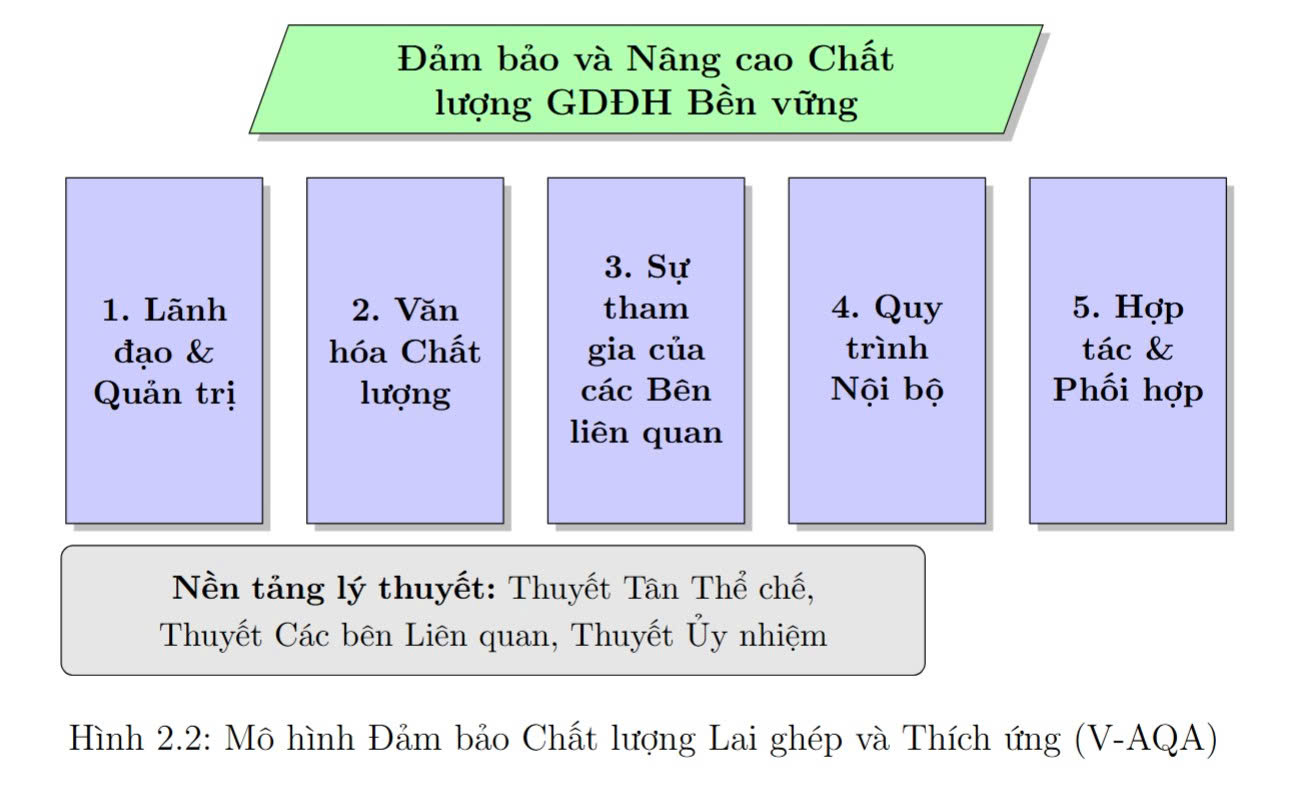
\includegraphics[width=0.9\textwidth]{image/mo_hinh_V-AQA.jpg}
    \caption{混合与适应性质量保障模型 (V-AQA)}
    \label{fig:v-aqa-model-detailed}
\end{figure}

\subsubsection{要素1的详细分析:领导与治理 (Leadership \& Governance)}
\label{subsubsec:thanh_to_1}

\paragraph{定义与范围:}
领导与治理要素是整个质量保障体系的源头,为之指明方向并提供资源。它不仅是行政管理活动,更是领导层在构建愿景、激发灵感以及建立有效治理结构以实现该愿景的能力。在越南的背景下,该要素包括校董会、校领导班子以及各级院、处、室领导的作用。它通过颁布关于质量的战略、政策及执行这些政策的承诺来体现。

\paragraph{理论与实践基础:}
该要素受到\textbf{委托代理理论}和\textbf{新制度主义理论}的强烈映射。
\begin{itemize}
    \item 从委托代理理论的角度看,学校领导层既是上级管理机构(教育培训部)的\textit{代理人},有责任执行国家政策;又是下级单位(院、系)的\textit{委托人},有责任监督并确保这些单位有效运作。明确的治理结构和责任划分是解决内部代理问题的先决条件。
    \item 从新制度主义的角度看,领导者是“解读”并诠释来自制度场域压力的角色。他们决定学校的战略:是被动遵守、模仿成功模式,还是主动寻求独特道路以创造差异化和独特的合法性。领导者的愿景将塑造学校与外部环境互动的方式。
\end{itemize}

\paragraph{实践中的指标与表现:}
为了评估一所大学在该要素上的发展水平,可以考察以下指标:
\begin{itemize}
    \item 是否存在一份详细的校级\textit{质量战略},并将其融入学校的总体发展战略中。
    \item 校领导班子、校董会涉及质量保障问题的会议频率和内容。
    \item 为质量保障活动分配资源(财务、人力)的程度。
    \item 规定质量保障相关单位职能、任务的文件的明确性。
    \item 关于干部、教师对领导层在质量工作中的承诺和导向作用的意见调查结果。
\end{itemize}
对这些指标的分析将在本论文的现状章节中详细进行。

% done chuong 2 goi 5
























